\chapter{Empirický model}
\section{Teoretické okénko}

První ze dvou měření mělo za cíl změřit závislost útlumu na vzdálenosti v husté městské zástavbě. Pro toto měření a následné modelování a realizaci v dlouhých, rovných ulicích v blízkosti FEL ČVUT, jsme použili One Slope Model, který je daný rovnicí 
\begin{equation}
    \overline{L(d)} = \overline{L_1(d_1)} + 10 n \log \big ( \frac{d}{d_1}\big),
\end{equation}
kde $\overline{L_1(d_1)}$ je útlum v referenční vzdálenosti $d_1$ v metrech a $n$ představuje parametr modelu závislý na typu prostředí.

Dále jsme zjišťovali standardní odchylku dat od průměrné hodnoty, neboli Log-Normal Shadowing. Výsledný model tak odpovídal vztahu 
\begin{equation}
    L(d) = \overline{L(d)} + X_\sigma = \overline{L_1(d_1)} + 10 n \log \big ( \frac{d}{d_1}\big) + X_\sigma,
\end{equation}
kde $\sigma$ je odchylka naměřených dat, zatímco $X_\sigma$ je útlum získaný z kumulativní distribuční funkce normálního rozdělení s daným $\sigma$.

Dále je třeba se zabývat i analýzou Fresnelova zlomu. Ten je dán vztahem
\begin{equation}
    d_0 = 4\frac{h_1 h_2}{\lambda},
\end{equation}
kde $h_1$, respektive $h_2$ jsou výšky antén a $\lambda$ je vLnová délka. Pokud se všechny veličiny dosadí v metrech, dostaneme výsledek také v metrech.

\section{Měření 1. - ulice Jugoslávských partyzánů}
Naše skupina si vybrala měření ve venkovním prostředí uvnitř husté městské zástavby. První měření probíhalo v ulici Jugoslávských partyzánů. Začátek byl na rohu s ulicí Rooseveltova, tam ostatně také byla umístěna vysílací anténa. Konec měření byl na konci náměstí Interbrigády. Celková trasa činila 370 metrů. 

Přijímací anténa s přístrojem byla přenášena v rámci trasy rychlostí asi 5 km/h -tedy poměrně klidnou lidskou chůzí. Obě antény byly umístěny ve výšce 170 cm nad zemí. Vysílací anténa byla umístěna na stativu, druhou bylo hýbáno po přímce.  Měření probíhalo v čase, kdy bylo na ulici poměrně rušno, tudíž bylo prakticky nemožné udržet s anténou po celou dobu přímou viditelnost. Celé měření pak trvalo asi 4 minuty.
Měření v této lokaci bylo provedeno dvakrát, jednou při pohybu od antény, podruhé při pohybu k anténě.
Grafy níže zachycují průběh jednoho měření, protože rozdíl od druhého měření nebyl tak velký. Výsledný model s parametry  $L_1$,  $\sigma$ a $n$ je tedy průměrem z jednotlivých výsledků měření.
Zjištěné hodnoty parametru $n$ odpovídají očekávaným hodnotám pro prostředí s hustou zástavbou.

\begin{table}[h!]
\centering
\begin{tabular}{|c|c|c|c|}
  \hline
   & Měření při pohybu od antény & Měření při pohybu k anténě & Průměr-Výsledný model \\
  \hline
  $L_1$ & 47,53 dB & 42,36 dB & 44,94 dB\\
  \hline
  n & 4,81 & 4,59 & 4,70 \\
  \hline
  $\sigma$ & 4.64 dB & 4.35 dB & 4,49 dB\\
  \hline
\end{tabular}
\caption{Přehled parametrů pro Měření I}
\end{table}

Vyjdeme-li z rovnice 1.3, tak zjistíme, že pro náš případ s uvedenými výškami antén a frenkvencí vychází, že vzdálenost Fresnelova zlomu je 38.5 metru. Proto budeme brát naměřené hodnoty až za touto vzdáleností. 
\subsection{Fotografie a záznamy hodnot z měření}

\begin{figure}[h!]
    \centering
    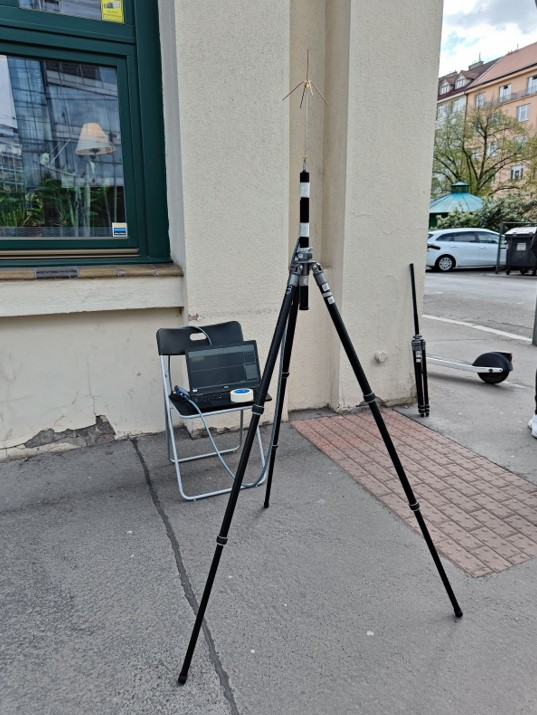
\includegraphics[,scale=0.55]{img/antenna_1.jpg}
    \caption{Vysílací stanoviště na rohu ulic Jugoslávských partyzánů a Roosveltova}
    \label{fig:my_label}
\end{figure}
\clearpage
\begin{figure}[h!]
    \centering
    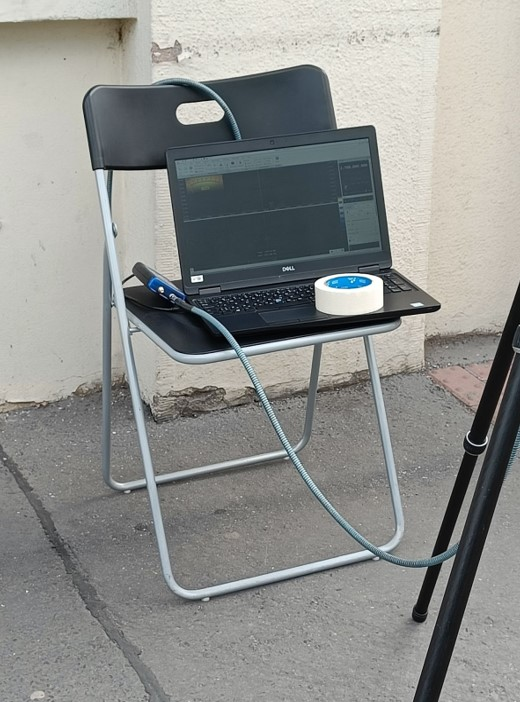
\includegraphics[,scale=0.4]{img/notebook_mereni1.jpg}
    \caption{Detail na umístění notebooku, včetně zapojení SDR}
    \label{fig:my_label}
\end{figure}



\begin{figure}[h!]
    \centering
    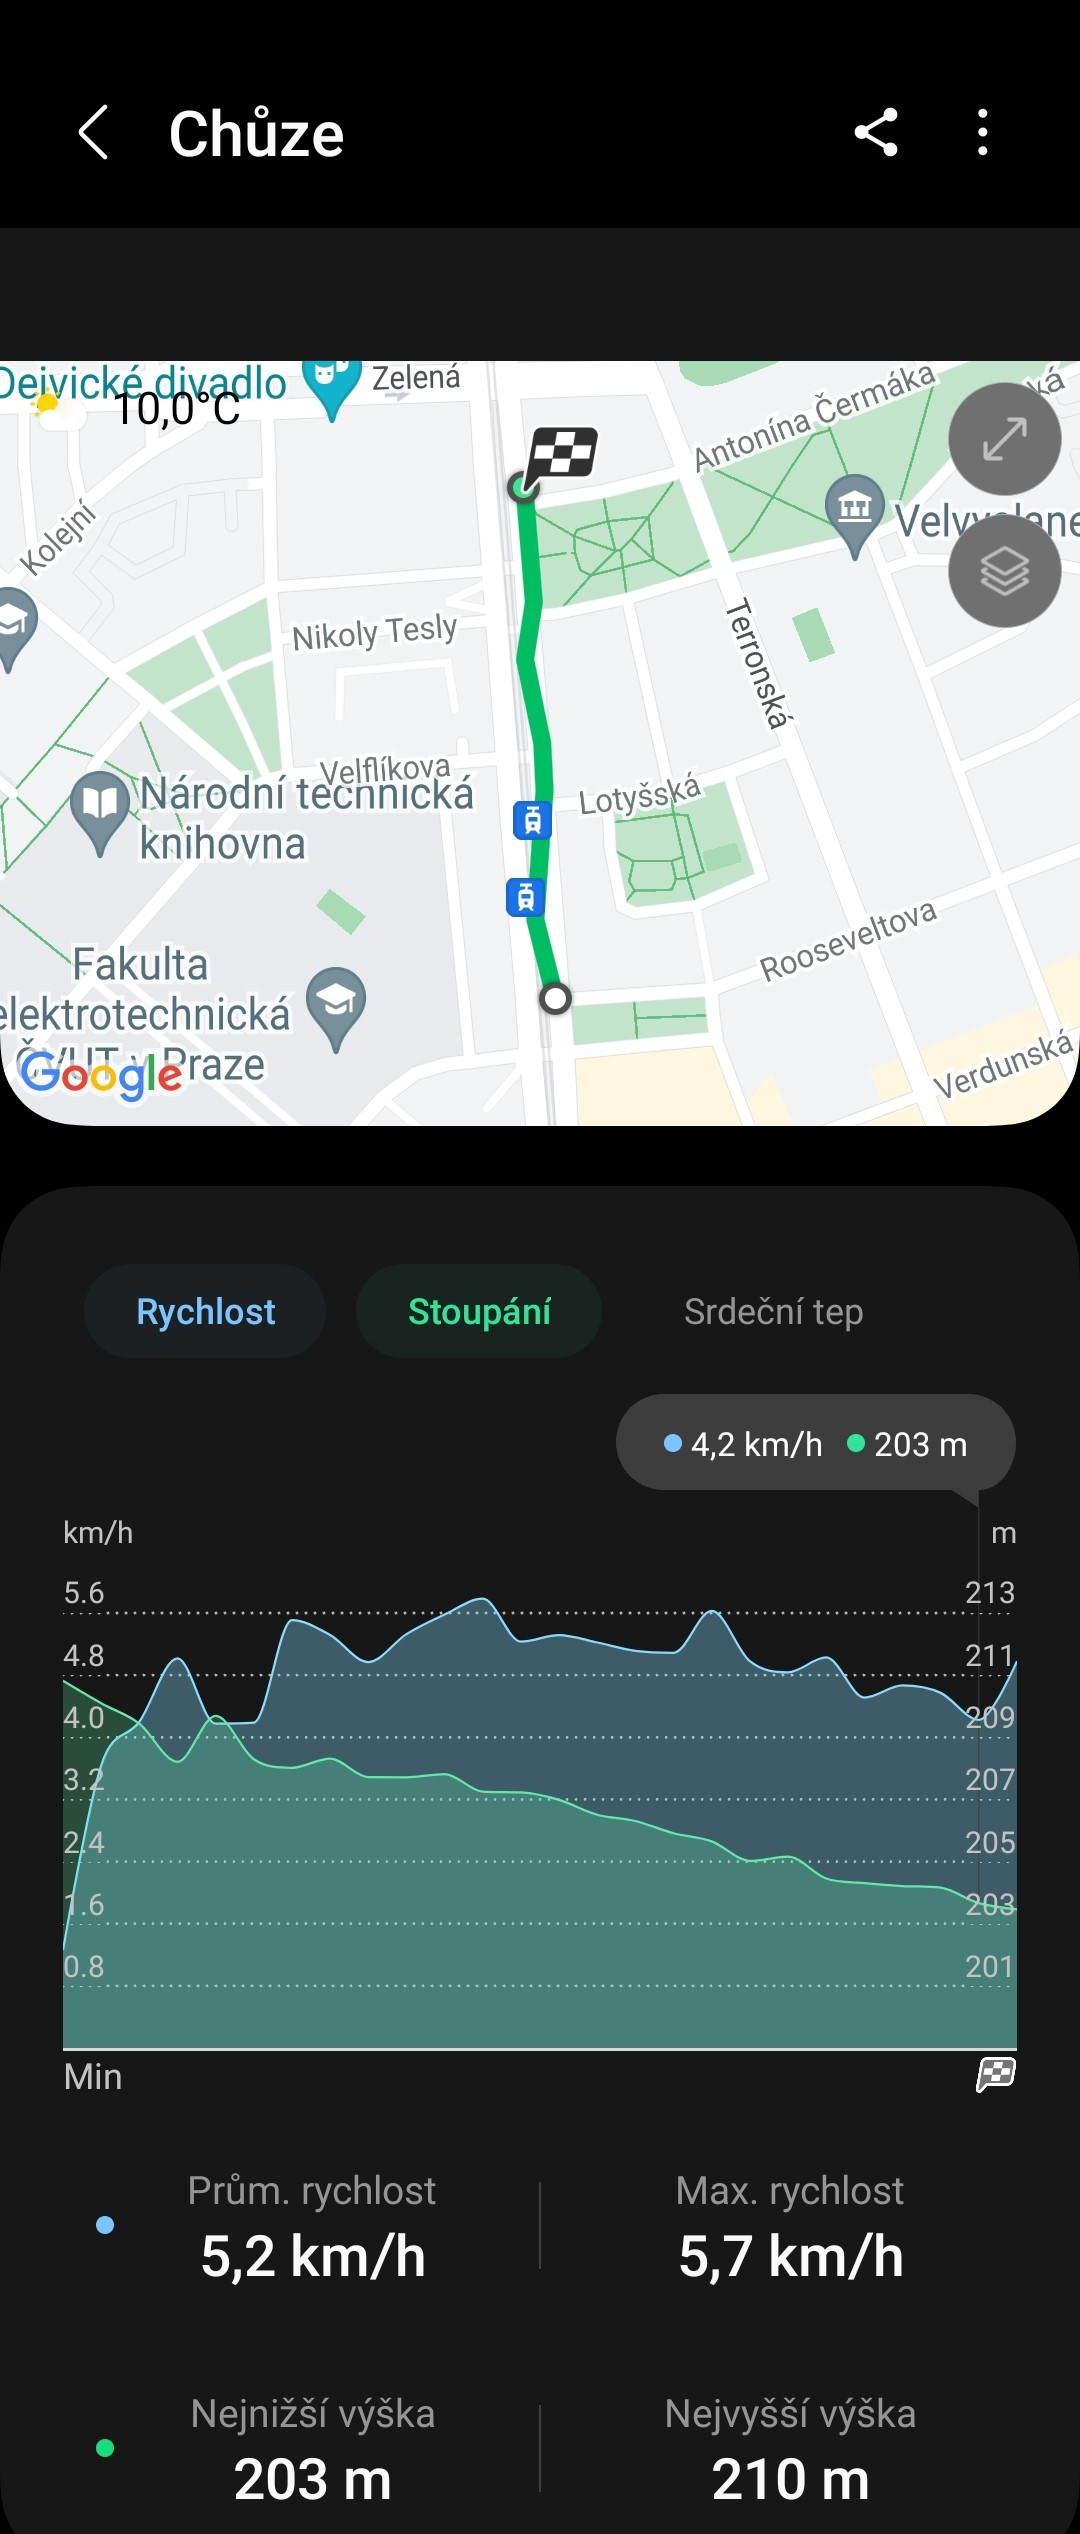
\includegraphics[,scale=0.16]{img/mereni1_cesta_tam.jpg}
    \caption{Data o vzdálenosti z GPS v mobilní aplikaci včetně rychlosti a převýšní}
    \label{fig:my_label}
\end{figure}
\clearpage
\begin{figure}[h!]
    \centering
    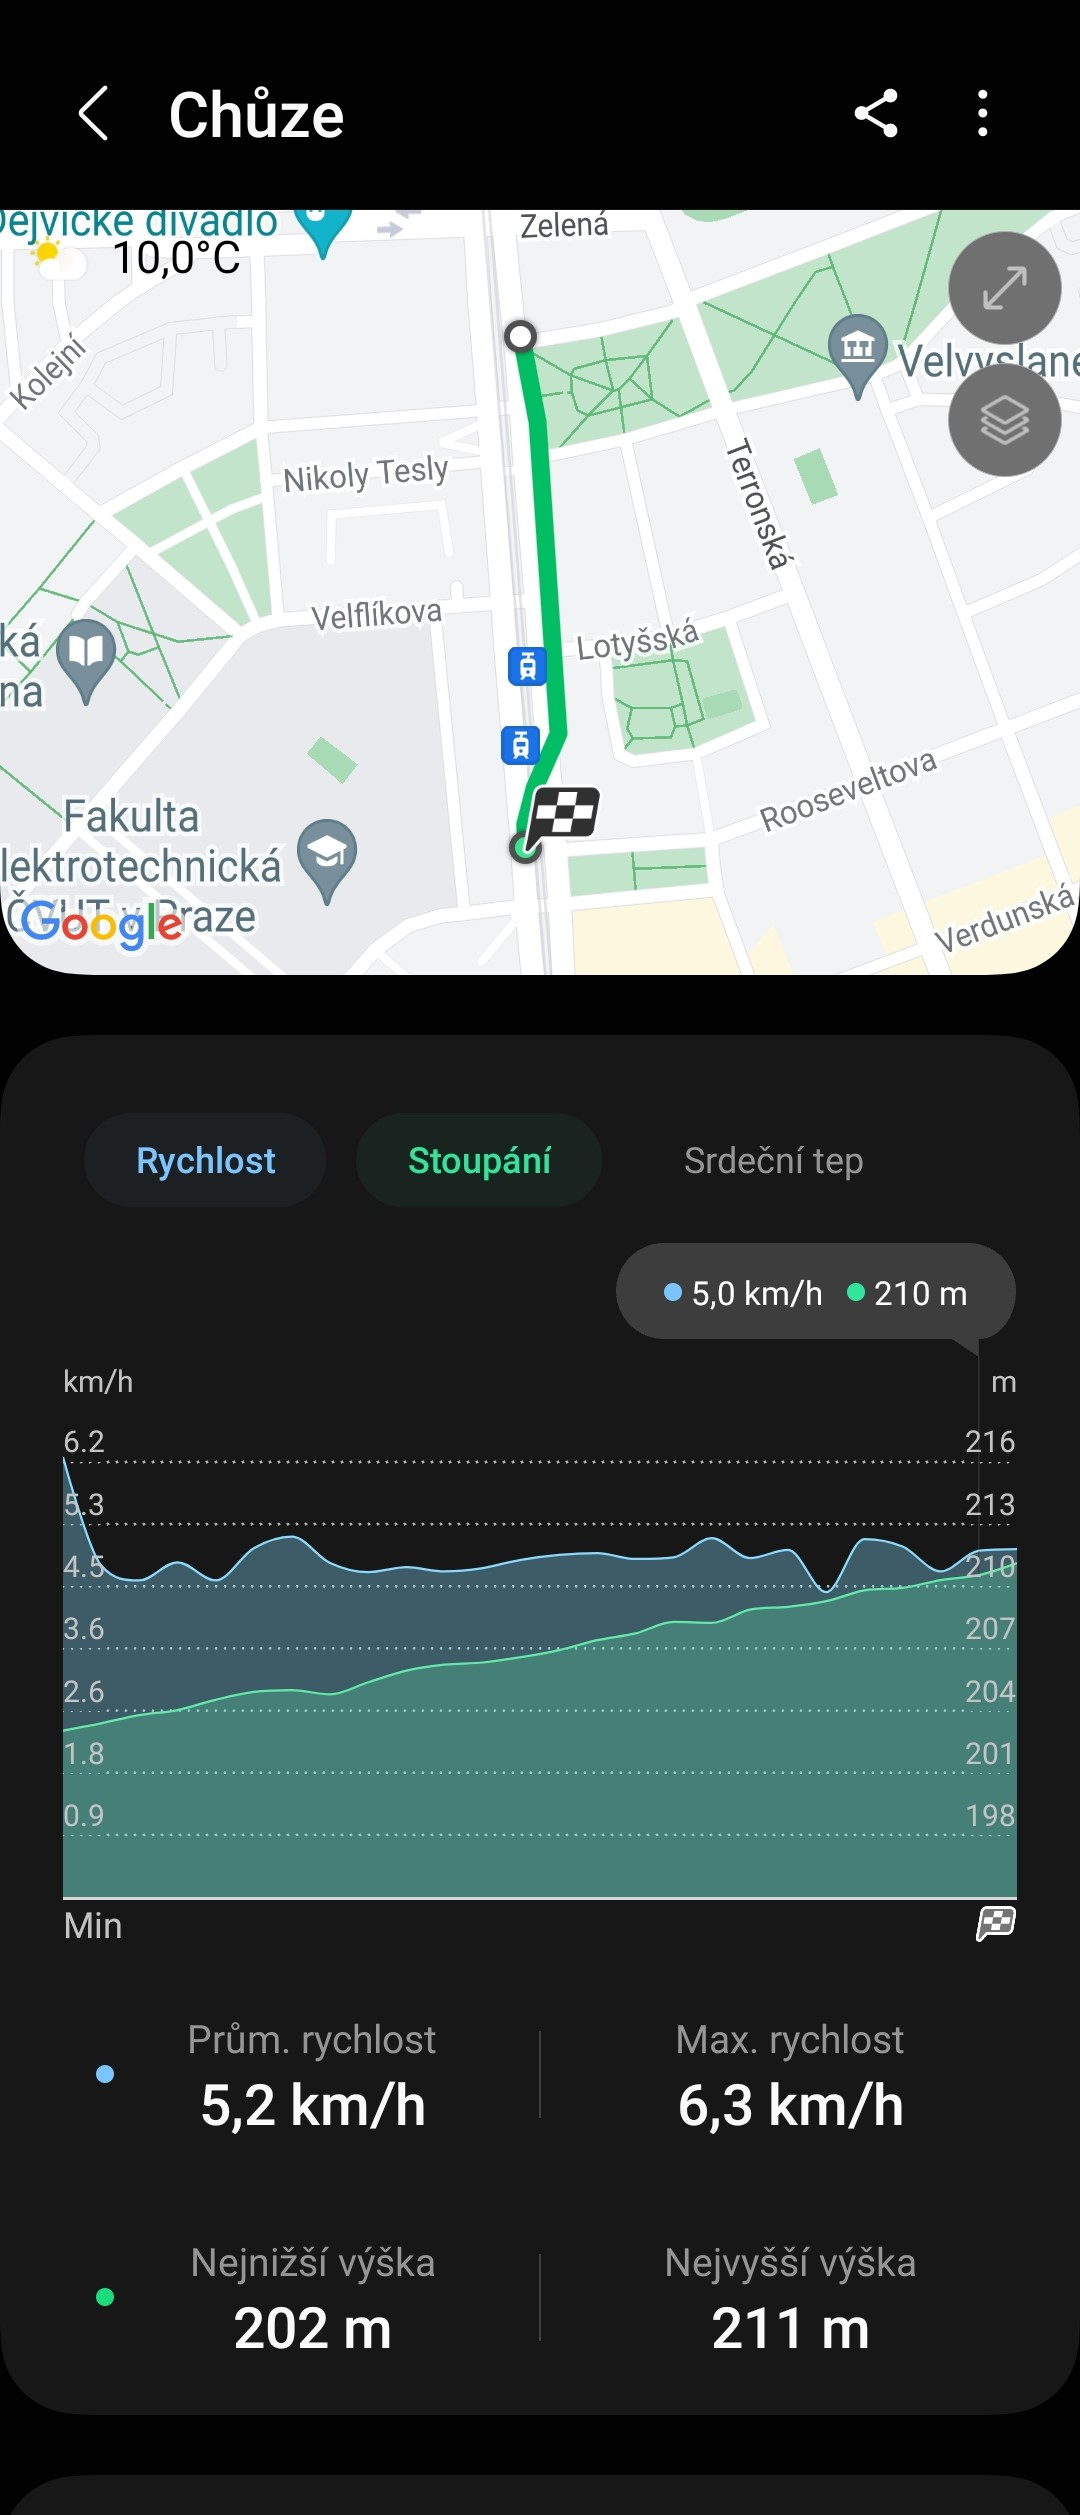
\includegraphics[,scale=0.16]{img/mereni1_Cesta_zpet.jpg}
    \caption{Data o vzdálenosti z GPS v mobilní aplikaci včetně rychlosti a převýšní pro cestu k vysílací anténě}
    \label{fig:my_label}
\end{figure}

\begin{figure}[h!]
    \centering
    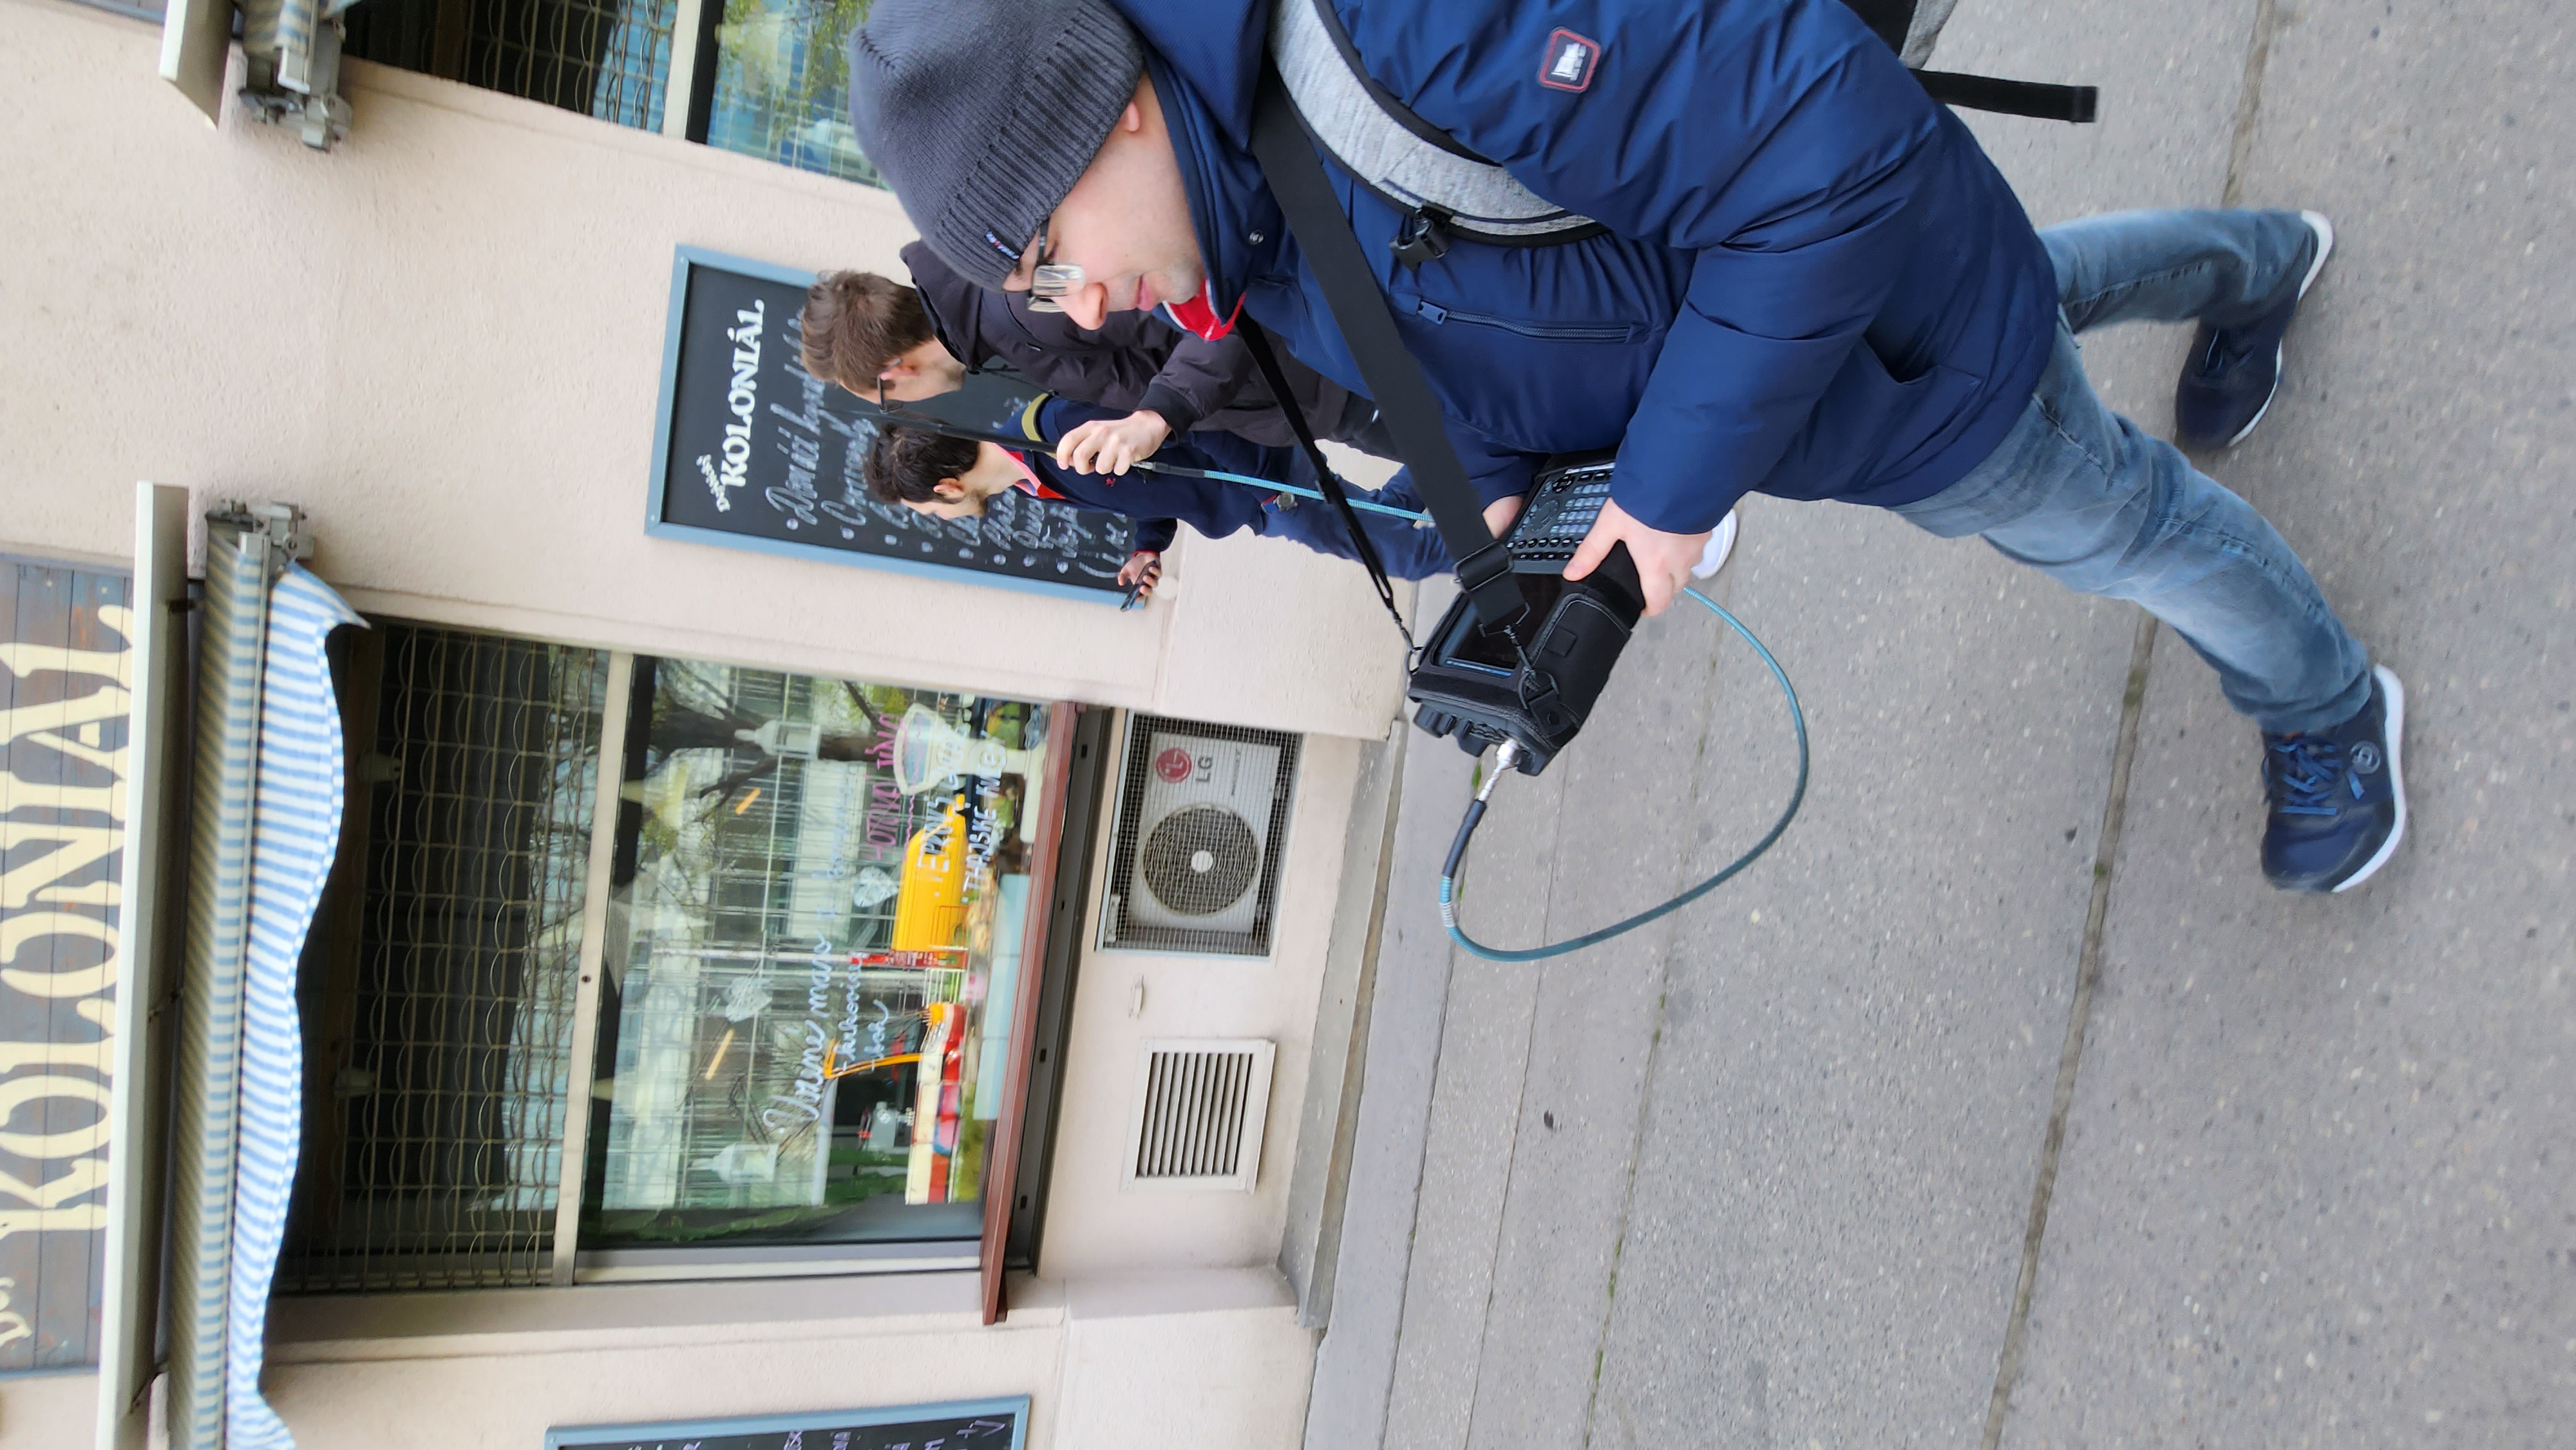
\includegraphics[angle=270,scale=0.07]{img/foto_mereni_jugoslavskych_partyzanu.jpg}
    \caption{Foto z průběhu měření v ulici Jugoslávských partyzánů}
    \label{fig:my_label}
\end{figure}

\subsection{Grafy s výsledky prvního měření}

Pro přehlednost celé práce jsou zde uvedeny grafy pouze pro měření v jednom směru. Výsledné hodnoty modelu jsou pak zprůměrováním obou měření v dané lokalitě. 

\begin{figure}[h!]
    \centering
    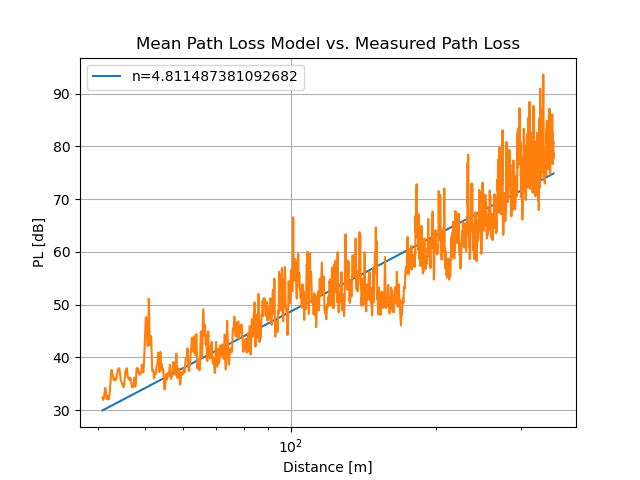
\includegraphics[,scale=0.8]{img/Mean_Path_LossVMeasured_partyzanu_dolu.png}
    \caption{Naměřená data a průběh emperického modelu}
    \label{fig:my_label}
\end{figure}

\begin{figure}[h!]
    \centering
    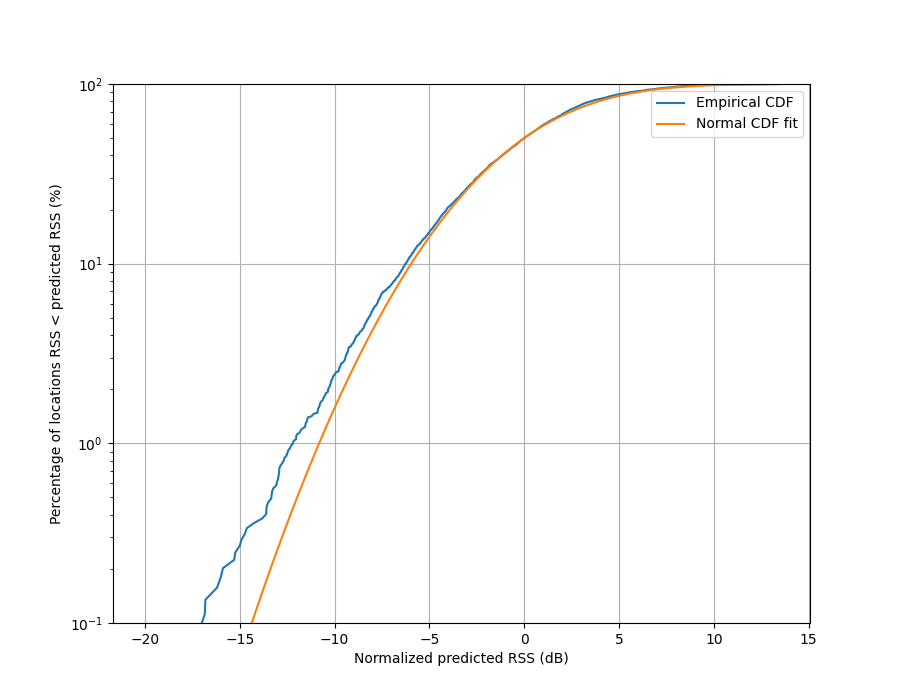
\includegraphics[,scale=0.52]{img/Prediction1_partyzanu_dolu.png}
    \caption{Graf zobrazující emperickou CDF a odhadnutou CDF}
    \label{fig:my_label}
\end{figure}

\begin{figure}[h!]
    \centering
    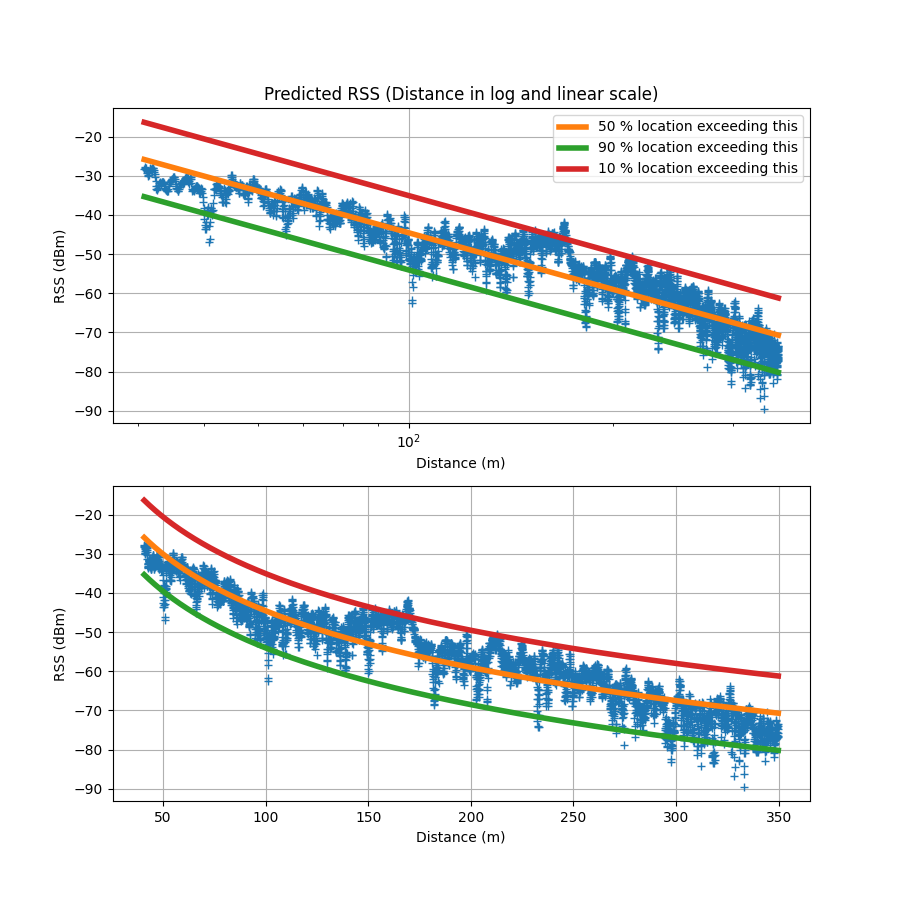
\includegraphics[,scale=0.52]{img/Prediction2partyzanu_dolu.png}
    \caption{Naměřená data společně s predikovaným průběhem modelu}
    \label{fig:my_label}
\end{figure}

\begin{figure}[h!]
    \centering
    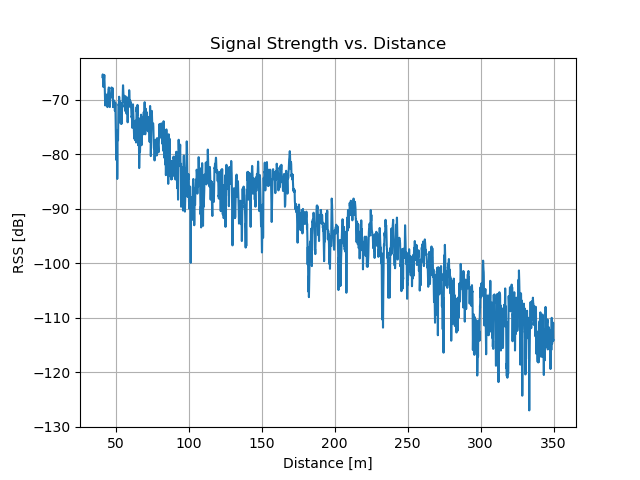
\includegraphics[,scale=0.7]{img/Signal_StrengthVDistance_partyzanu_dolu.png}
    \caption{Naměřené hodnoty síly signálu v závislosti na vzdálenosti}
    \label{fig:my_label}
\end{figure}

\begin{figure}[h!]
    \centering
    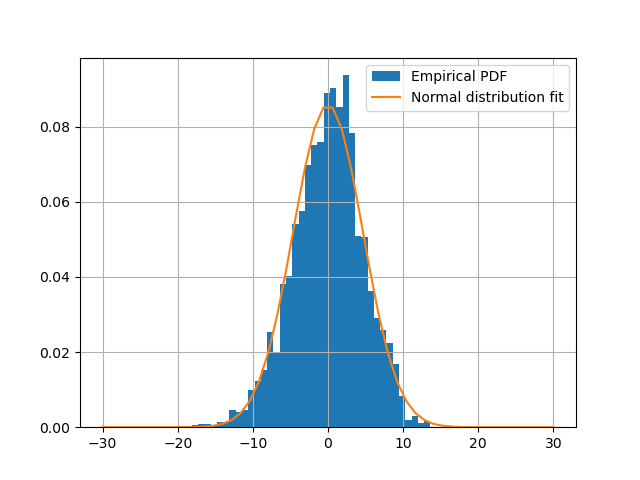
\includegraphics[,scale=0.7]{img/Statistics_partyzanu_dolu.png}
    \caption{Normálové rozdělí a jeho porovnání s rozdělením naměřených dat}
    \label{fig:my_label}
\end{figure}

\section{Měření 2. - ulice Teronská}
Druhé měření bylo také provedeno uvnitř husté zástavby, tentokrát v ulici Terronská. Měření bylo usutečněno od rohu ulice Rooseveltova na roh ulice Antonína Čermáka, kde celková trasa má 370 metrů. Výšky antén byly umístěny ve stejné výšce jako v prvním měření, tedy 170 cm nad zemí. Metodika měření byla stejná jako v 1. měření. Tato trasa se jeví jako lepší z důvodu menší rušnosti. Prakticky po celou dobu měření byla přímá viditelnost mezi jednotlivými anténami. Měření v této lokaci bylo provedeno dvakrát, jednou při pohybu od antény, podruhé při pohybu k anténě. 
V záznamu trasy dle GPS je celková délka 370 metrů.
Protože je ale celková trasa mírně z kopce a na posledních několika desítkách metrech už převýšení není, navíc se tam nachází park, jsme se rozhodli posledních asi 170 metrů při zpracování měření vyřadit, tak aby měření odpovídalo měření v husté městské zástavbě a nebylo ovlivněno terénem. Z toho důvodu následují grafy končí se vzdáleností 200 metrů.
Grafy níže zachycují průběh jednoho měření, protože rozdíl od druhého měření nebyl tak velký. Výsledný model s parametry  $L_1$,  $\sigma$ a $n$ je tedy průměrem z jednotlivých výsledků měření.
Zjištěné hodnoty parametru $n$ odpovídají očekávaným hodnotám pro prostředí s hustou zástavbou.


\begin{table}[h!]
\centering
\begin{tabular}{|c|c|c|c|}
  \hline
   & Měření při pohybu od antény & Měření při pohybu k anténě & Průměr-Výsledný model \\
  \hline
  $L_1$ & 44,72 dB & 31,06 dB & 37,89 dB\\
  \hline
  n & 4,62& 4,06 & 4,34 \\
  \hline
  $\sigma$ & 4,39 dB & 4,34 dB & 4,36 dB \\
  \hline
\end{tabular}
\caption{Přehled parametrů pro měření v ulici Terronská}
\end{table}

Vyjdeme-li z rovnice 1.3, tak zjistíme, že pro náš případ s uvedenými výškami antén a frenkvencí vychází, že vzdálenost Fresnelova zlomu je opět 38.5 metru., protože jsme vysílali na stále stejné frekvenci a ani výška antén se zde neměnila. 
\subsection{Fotografie a záznamy hodnot z měření}

\begin{figure}[h!]
    \centering
    \includegraphics[angle=270,scale=0.06]{img/antena_terronska.jpg}
    \caption{Vysílací stanoviště v ulici Terronská s pohledem ve směru měření}
    \label{fig:my_label}
\end{figure}

\begin{figure}[h!]
    \centering
    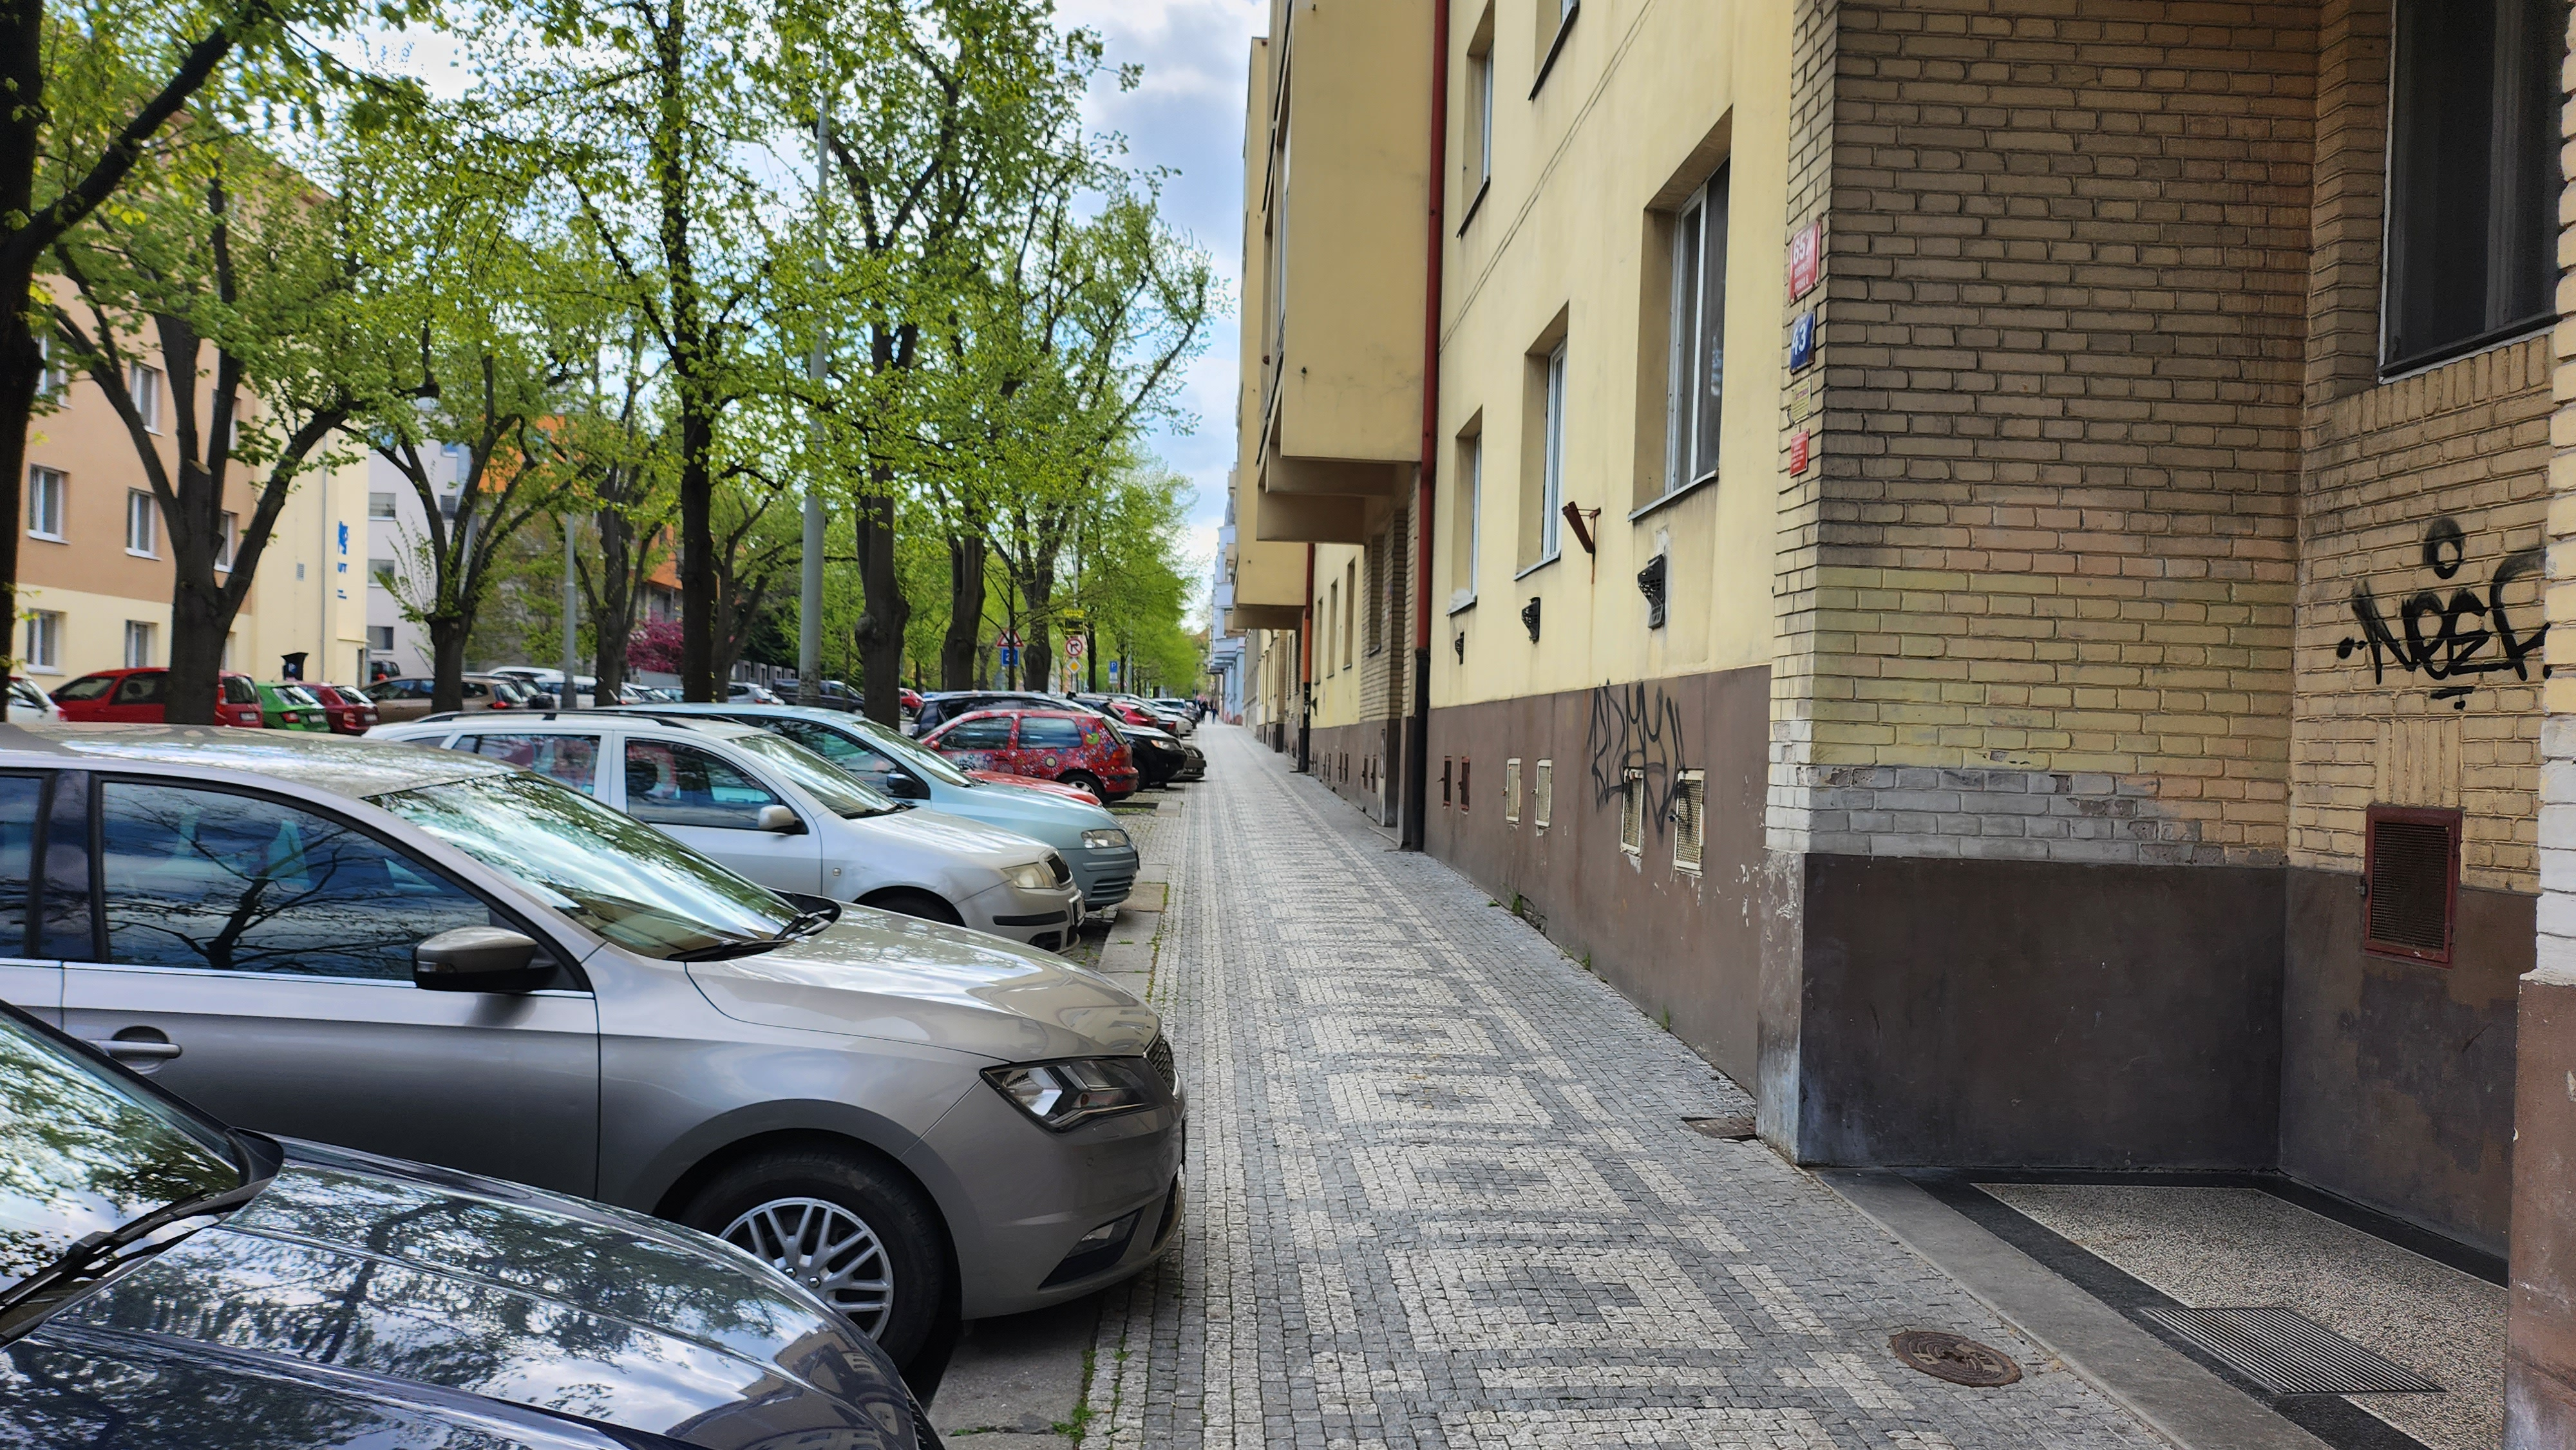
\includegraphics[,scale=0.06]{img/pohled_terronska.jpg}
    \caption{Ulice Terronská směrem k vysílací anténě}
    \label{fig:my_label}
\end{figure}

\clearpage

\begin{figure}[h!]
    \centering
    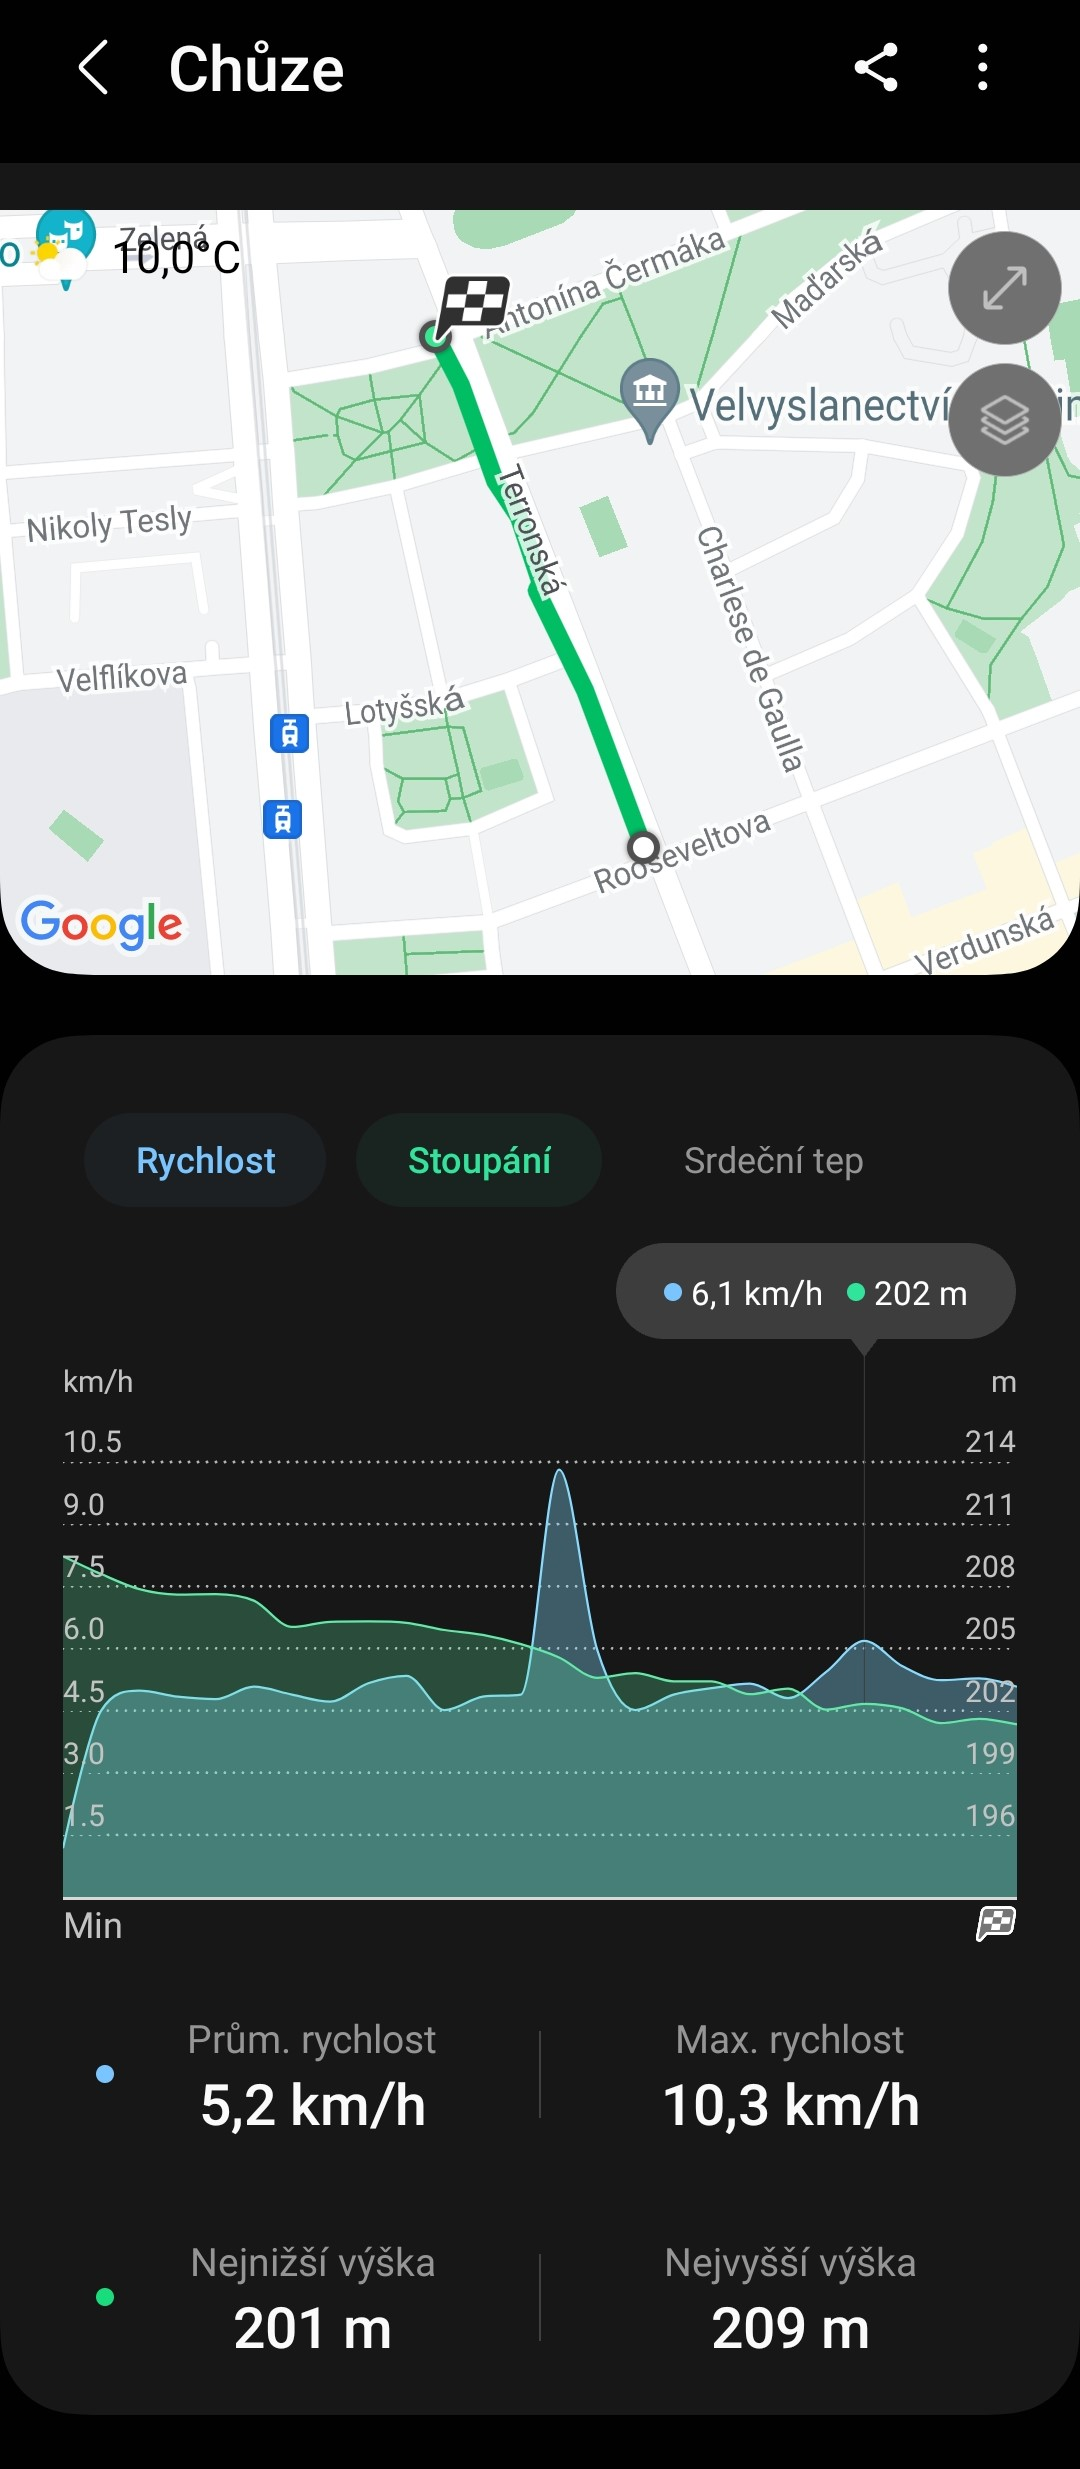
\includegraphics[,scale=0.16]{img/terronska_cestaTam.jpg}
    \caption{Data o vzdálenosti z GPS v mobilní aplikaci včetně rychlosti a převýšní}
    \label{fig:my_label}
\end{figure}

\begin{figure}[h!]
    \centering
    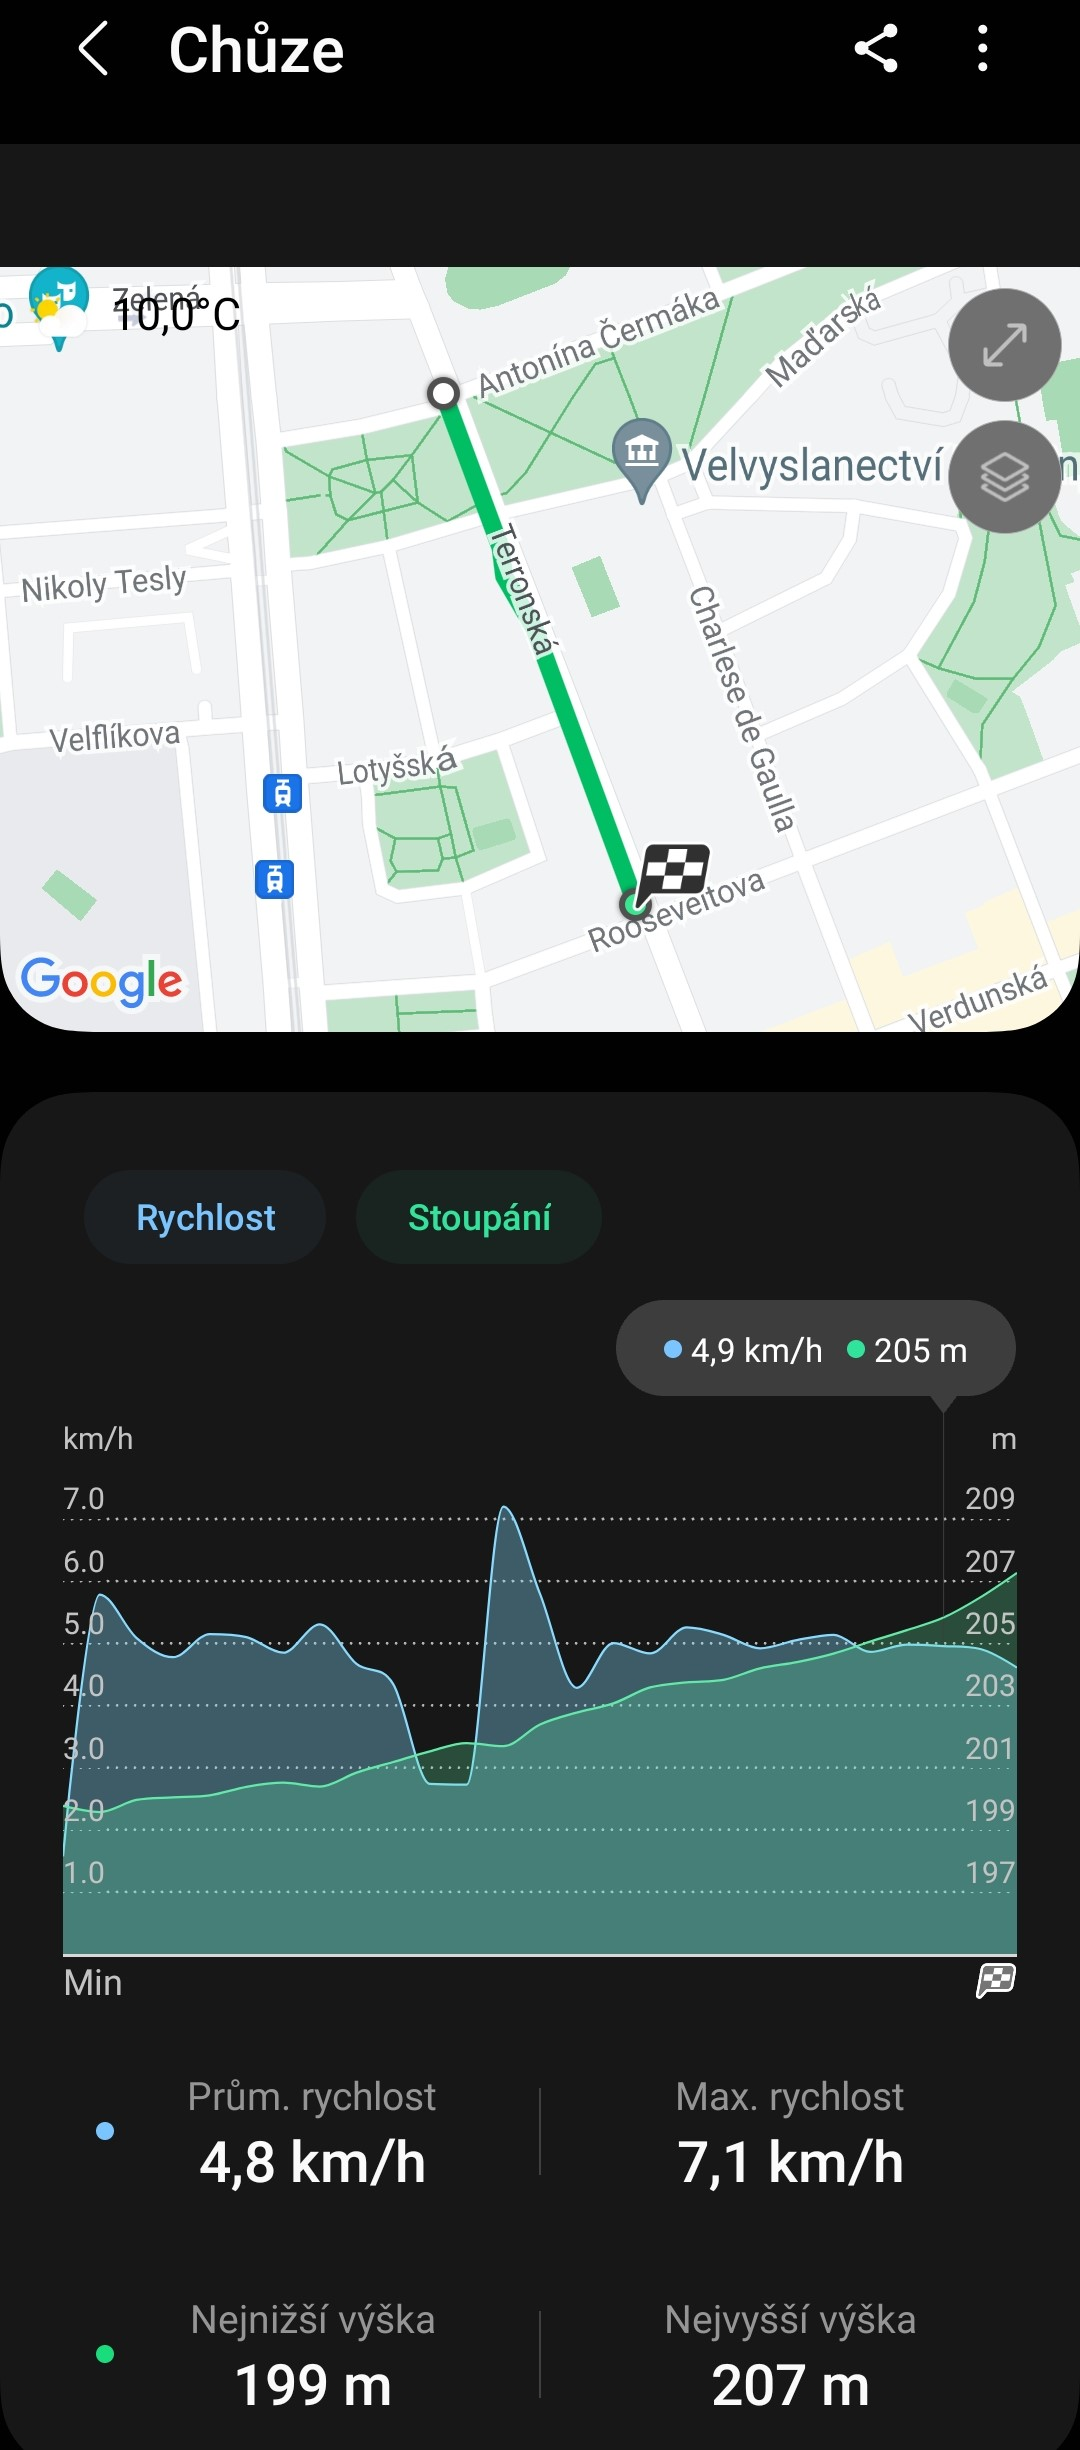
\includegraphics[,scale=0.16]{img/terronska_cesta_zpet.jpg}
    \caption{Data o vzdálenosti z GPS v mobilní aplikaci včetně rychlosti a převýšní pro cestu k vysílací anténě}
    \label{fig:my_label}
\end{figure}

\begin{figure}[h!]
    \centering
    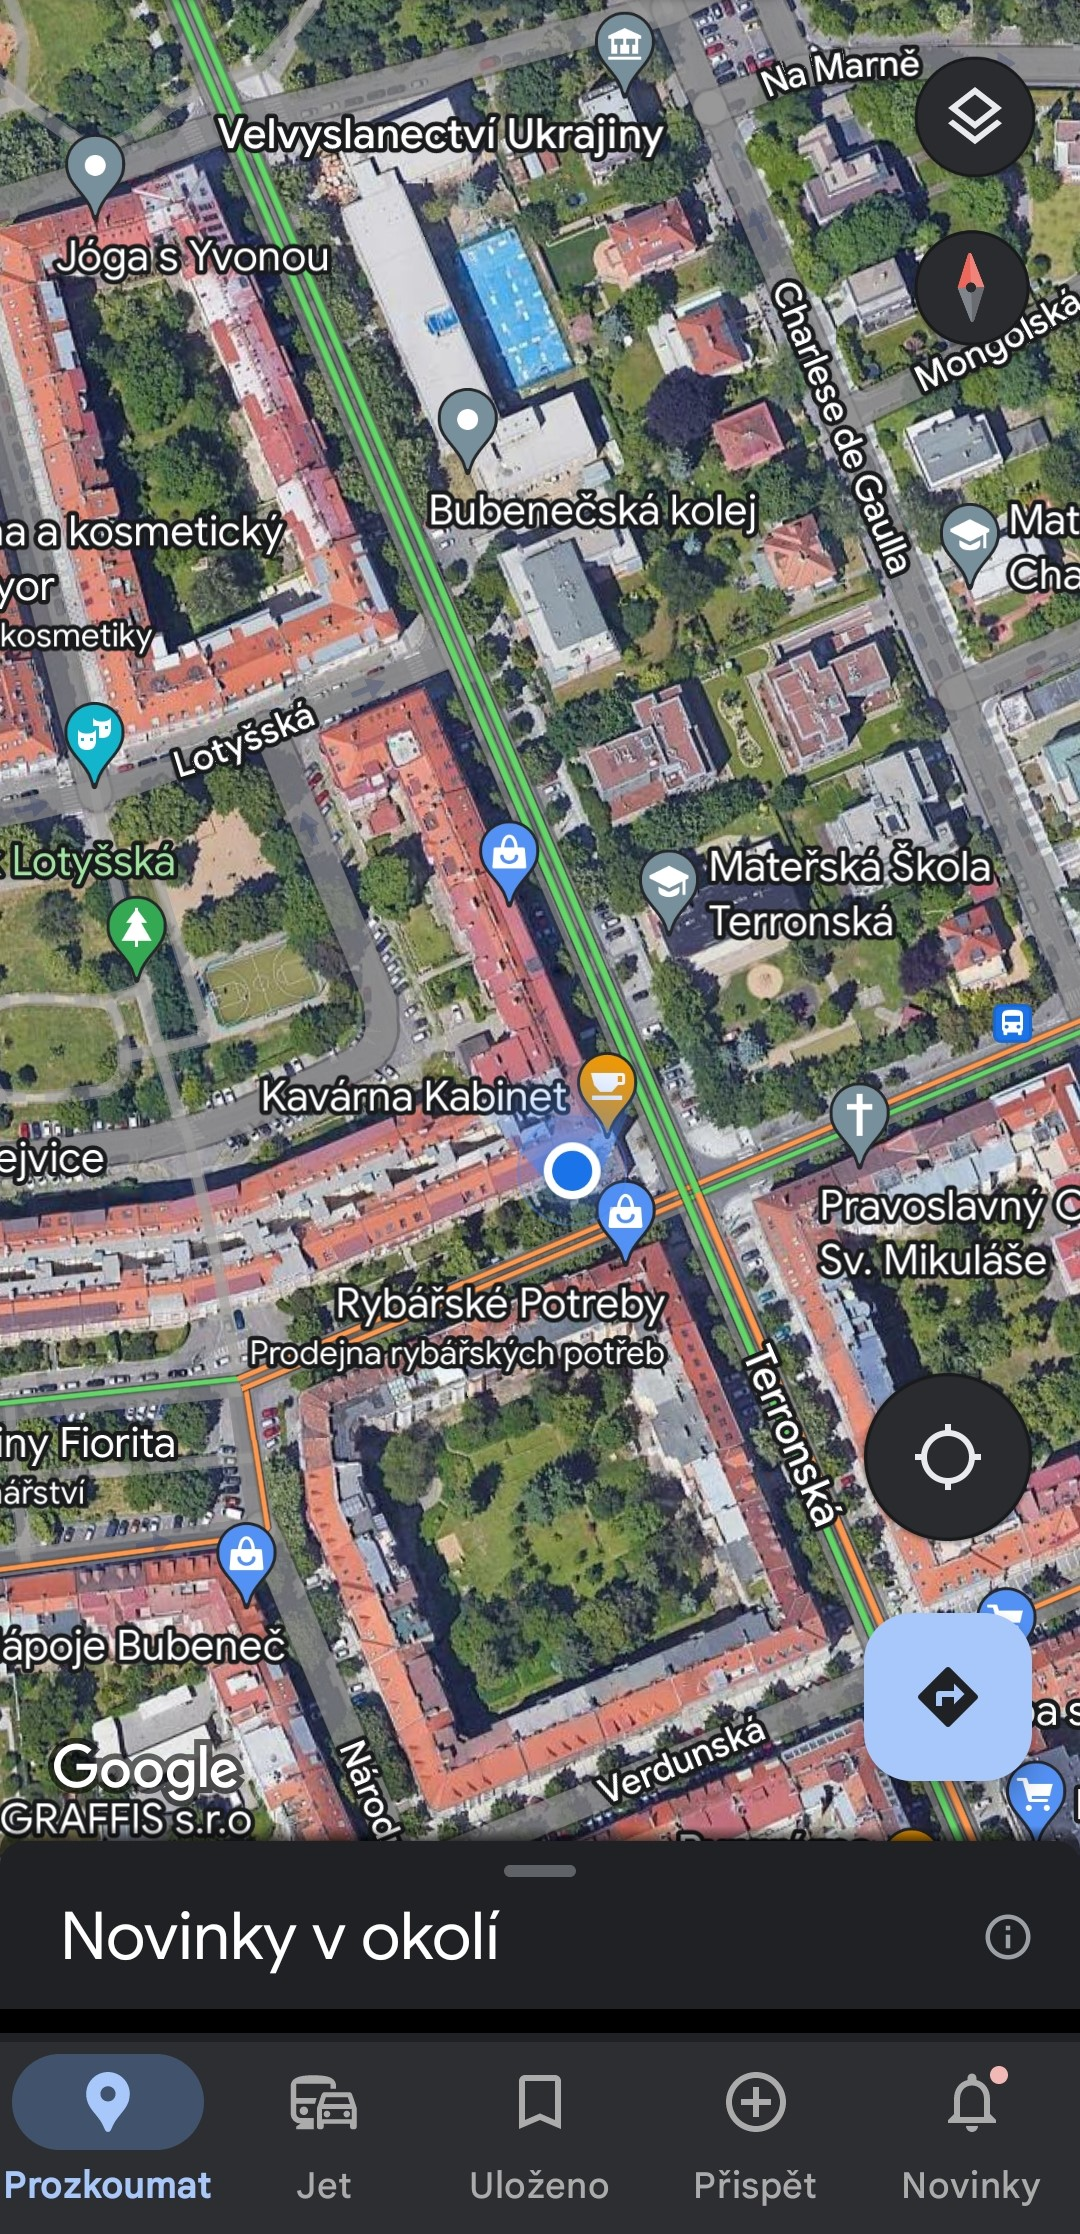
\includegraphics[,scale=0.16]{img/terronska_Satelitnisnimek.jpg}
    \caption{Satelitní snímek měřené trasy s hrubým poznačením vysílací antény}
    \label{fig:my_label}
\end{figure}

\subsection{Grafy s výsledky druhého měření}

Pro přehlednost celé práce zde opět uvádíme pouze grafy vztažené k měření při pohybu přijímací antény směrem od vysílače (jako i pro měření v ulici Jugoslávských partyzánů). Výsledné hodnoty modelu jsou pak zprůměrováním obou měření v dané lokalitě.


\begin{figure}[h!]
    \centering
    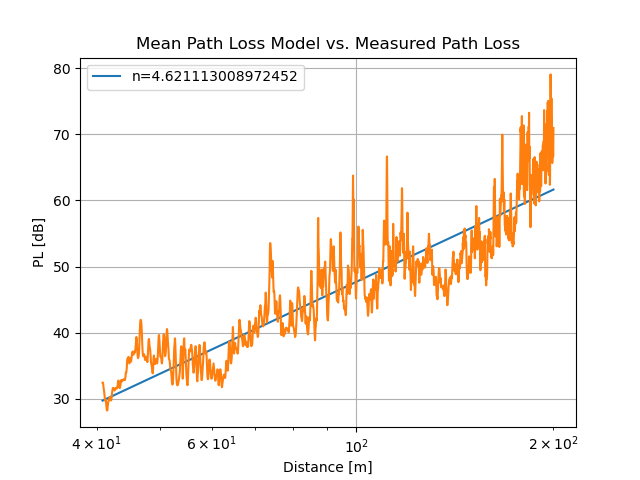
\includegraphics[,scale=0.75]{img/Mean_Path_LossVMeasured_terronska_dolu.png}
    \caption{Naměřená data a průběh emperického modelu}
    \label{fig:my_label}
\end{figure}

\begin{figure}[h!]
    \centering
    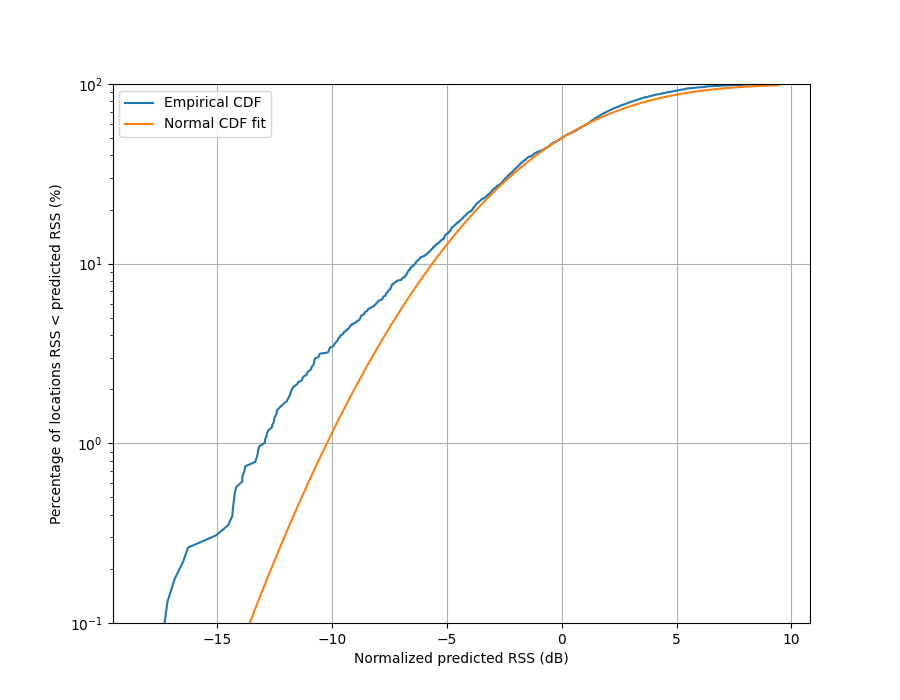
\includegraphics[,scale=0.52]{img/Prediction1_terronska_dolu.png}
    \caption{Graf zobrazující emperickou CDF a odhadnutou CDF}
    \label{fig:my_label}
\end{figure}

\begin{figure}[h!]
    \centering
    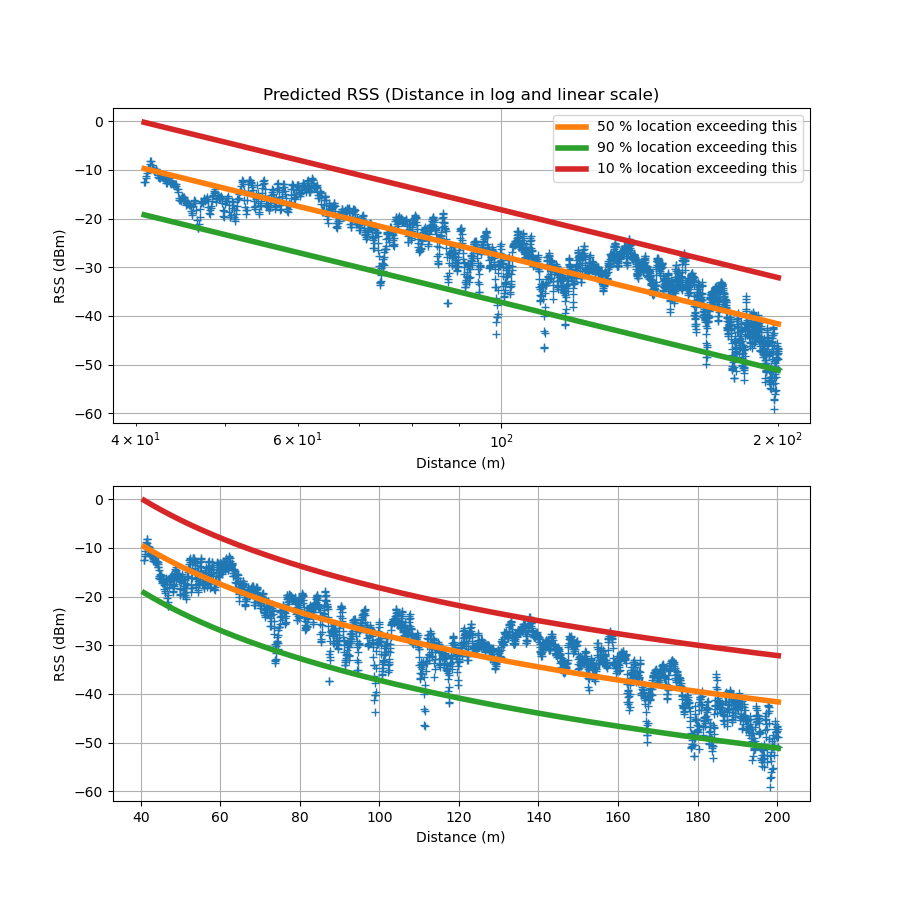
\includegraphics[,scale=0.52]{img/Prediction2terronska_dolu.png}
    \caption{Naměřená data společně s predikovaným průběhem modelu}
    \label{fig:my_label}
\end{figure}

\begin{figure}[h!]
    \centering
    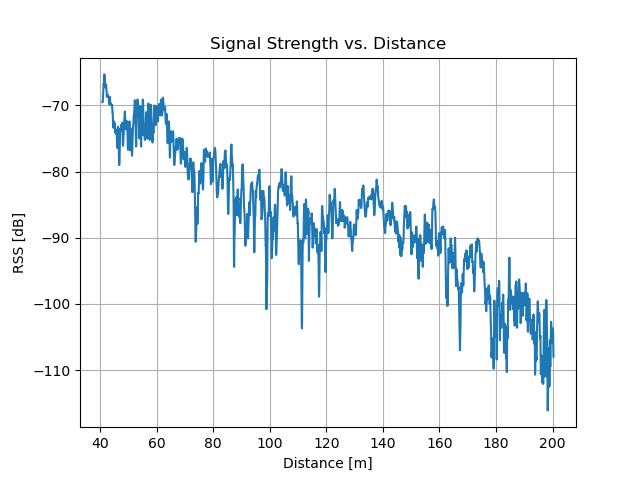
\includegraphics[,scale=0.7]{img/Signal_StrengthVDistance_terronska_dolu.png}
    \caption{Naměřené hodnoty síly signálu v závislosti na vzdálenosti}
    \label{fig:my_label}
\end{figure}

\begin{figure}[h!]
    \centering
    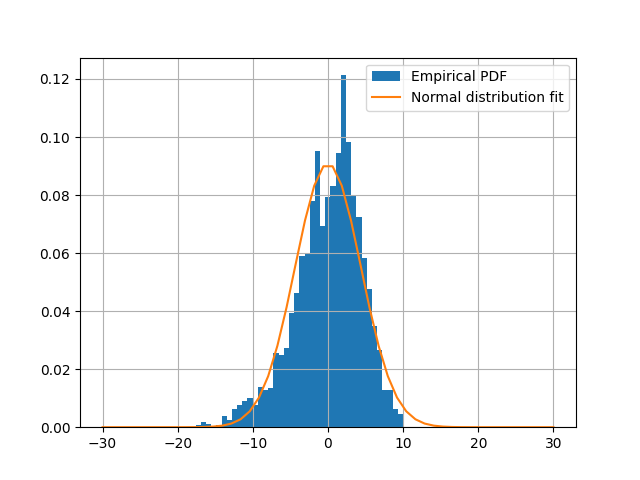
\includegraphics[,scale=0.7]{img/Statistics_terronska_dolu.png}
    \caption{Normálové rozdělí a jeho porovnání s rozdělením naměřených dat}
    \label{fig:my_label}
\end{figure}

\section{Shrnutí měření}
Při tomto měření jsme zjistili jak vzdálenost přijímače od vysílací antény ovlivňuje sílu signálu, která s rostoucí vzdáleností klesá. Změřené výsledky jsme byly dobře schopni proložit trendem a sestavit tak empirický model husté zástavby. Získané hodnoty parametru $n$ odpovídají teoretickým hodnotám pro městskou hustou zástavbu. 




